\documentclass[a4paper,26pt]{article}
\usepackage{geometry}                		% See geometry.pdf to learn the layout options. There are lots.
\geometry{letterpaper}                   		% ... or a4paper or a5paper or ... 
%\geometry{landscape}                		% Activate for rotated page geometry
%\usepackage[parfill]{parskip}    		% Activate to begin paragraphs with an empty line rather than an indent
\usepackage{graphicx}				% Use pdf, png, jpg, or eps§ with pdflatex; use eps in DVI mode	
\usepackage{amssymb}
\usepackage{xcolor,sectsty}
\usepackage{float}
\usepackage{authblk}
\usepackage[
backend=biber,
style=alphabetic,
citestyle=authoryear 
]{biblatex}
\addbibresource{report_bibliography.bib}
% One must be careful when importing hyperref. Usually it has to be the last package to be imported, but there might be some exceptions to this rule.
\usepackage{hyperref}
\usepackage{times}
\usepackage{epsfig}
\usepackage{graphicx}
\usepackage{amsmath}
\usepackage{amssymb}
\usepackage{subcaption}
\usepackage{multirow}
% Styles
\definecolor{astral}{RGB}{46,116,181}
% \subsectionfont{\color{astral}}
% \sectionfont{\color{astral}}

\urlstyle{same}

%SetFonts
\usepackage{etoolbox}

%SetFonts

\title{Sentiment Analysis using Word Vectors}

\author{ATJ}

\author{NSB}

\affil{University of Massachusetts, Amherst}

\date{}

\begin{document}

\maketitle

\pagenumbering{gobble}

\pagenumbering{arabic}

\begin{abstract}

For the task of sentiment analysis, a document can be represented in multiple forms - as a bag of words of unigram frequencies, as a bag of words of unigram absence/presence indicators, as a bag of words of bigram frequencies, or as word vectors generated from Latent Dirichlet Allocation (LDA), Latent Semantic Analysis (LSA), word2vec or doc2vec. The selection of a particular document representation is crucial to yield good accuracies in sentiment analysis. In this project we evaluate these different document representations over three widely available datasets - Review Polarity v2.0 dataset and the Subjectivity dataset provided by \cite{pang2004sentimental}, and the Large Movie Review Dataset v1.0 made available by \cite{maas2011learning} using a multitude of classifiers - Naïve Bayes, Logistic Regression, K-Nearest Neighbors, Decision Trees, Random Forests, Support Vector Machines and Ensemble classifiers. The results we obtained align with those obtained by \cite{maas2011learning}. We find that word vector representations using word2vec and doc2vec are the best document representations for sentiment analysis as they capture both semantic and sentiment information. 

\end{abstract}

\section{Introduction}

\paragraph{}

Sentiment Analysis is the task of extracting the favorable or unfavorable inclination of a person towards a subject or topic. For example, we could analyze twitter feeds to predict or assess the stock market trends, the favor-ability of a presidential nominee during elections, or how good a movie is based on the volume of the tweets and their content. It can be used to get user opinions on the products the user purchased based on the star ratings and reviews submitted through online portals like amazon.com which can be used by product manufacturers to identify how well their product is received by the majority of users. This kind of feedback is invaluable and very crucial in many cases. \textit{How can we represent a document so that we achieve high accuracies in sentiment analysis? What information would this representation capture?}

\paragraph{}

For the purpose of sentiment analysis, one could view a document as simply a ``bag of words'' in which the position of words does not matter. In addition, it ignores the semantics of the words. For example, it cannot capture the relationship between ``powerful'', ``strong'' and ``Paris''. Vector based models are able to capture the relational structure of the lexicon. Vector based models can represent words as distance or angle between word vectors in a high-dimensional space. This gives us ability to evaluate word similarities. Different word vectors capture different information about the documents. Some word vectors capture semantic information of the words, while other representations capture both semantic and sentiment information. The particular document representation selected for sentiment analysis has a huge impact on the accuracy of the classifier.

\paragraph{}
With automated review rating (opinion rating), advertisers could track advertising campaigns, politicians could track public opinion, reporters could track public response to current events, stock traders could track financial opinions, and trend analyzers could track entertainment and technology trends.
There are results from previous research that indicate humans may not always have the best intuition for choosing
discriminating words when expressing sentiment or writing reviews. 
Movie reviews are also found to be the most toughest of sentiment classification. 
What makes sentiment classification harder over topic classification or similar tasks is that it not just depends on the words present in a document but also on their arrangement,if not more so. The impression or review of a movie could be positive but if the description contains negative words like ``a bad person'' , ``most evil character'', ``insipid fellow'', the classification accuracy suffers because of the presence of words with negative sentiment. 

\paragraph{}

In this project, we evaluate some of these different document representations - bag of words using unigram frequencies, bag of words using unigram absenece/presence indicators, bag of words using bigrams, word vectors obtained from Latent Dirichlet Allocation (LDA) \cite{blei2003latent}, Latent Semantic Allocation (LSA), word2vec \cite{le2014distributed} and doc2vec using a multitude of classifiers such as Naïve Bayes, Logistic Regression, K-Nearest Neighbors, Decision Trees, Random Forests, Support Vector Machines and Ensemble classifiers. We evaluate these different document representations by training and testing the classifiers over three widely available datasets - Review Polarity v2.0 dataset and the Subjectivity dataset provided by \cite{pang2004sentimental}, and the Large Movie Review Dataset v1.0 made available by \cite{maas2011learning}. The accuracies that \cite{maas2011learning} and others \cite{sadeghianbag} reported on the three datasets are listed in Table \ref{table:1}. Our experiments similarly reveal that we can achieve high accuracies in sentiment analysis using word vector representations obtained from word2vec and doc2vec. 

\section{Related Work}

\paragraph{}
\cite{maas2011learning} present a model to capture both semantic and sentiment similarities among words.
The semantic component of their model learns word vectors via an unsupervised probabilistic model of documents like LDA or LSA. The semantic component does not include sentiment information in the word vectors. For example, while it learns that ``wonderful'' and ``amazing'' are semantically close, it doesn't capture the fact that these are both very strong positive
sentiment words, at the opposite end of the spectrum from ``terrible'' and ``awful''. They come up with an algorithm that through supervised learning adds sentiment information into the word vectors learnt above. The resultant vectors have similar representations for words that are similar in both semantic and sentimental context. They have tested their model on the three data sets we have proposed to use for our project against other bag of words and LDA, LSA document or word representations and evaluated the efficiency of their model. 

\begin{table}[H]
\begin{tabular}{ | l | p{1.5cm} | p{2.5cm} | p{2.5cm} |  }
 \hline
 \textbf{Features} & \textbf{PL04} & \textbf{IMDB Dataset} & \textbf{Subjectivity} \\
 \hline
 Bag of Words   & 85.45 & 87.80 & 87.77 \\

 LDA & 66.70 & 67.42 & 66.65 \\

 LSA & 84.55 & 83.96 & 82.82 \\
 \cite{maas2011learning}'s Semantic Only & 87.10 & 87.30 & 86.65 \\

 \cite{maas2011learning}'s Full & 84.65 & 87.44 & 86.19 \\

 \cite{maas2011learning}'s Full + Bag of Words (bnc) & 87.85 & 88.33 & 88.45 \\
 Bag of Words SVM \cite{pang2004sentimental} & 87.15 & N/A & 90.00 \\
 \hline
\end{tabular}
\caption{Classification accuracies reported by \cite{maas2011learning} and others for different word representations.}
\label{table:1}
\end{table}

\paragraph{}
Semantic vector spaces for single words have been widely used as features, but they cannot capture the meaning of longer phrases properly. To remedy this, \cite{socher2013recursive} introduce a Sentiment Treebank which includes fine grained sentiment labels for 215,154 phrases in the parse trees of 11,855 sentences. The corpus is based on the dataset introduced by \cite{pang2005seeing} and consists of 11,855 single sentences extracted from movie reviews. They also propose a new model of recurrent neural network called Recursive Neural Tensor Networks that can take as input phrases of any length. They represent a phrase through word vectors and a parse tree and then compute vectors for higher nodes in the tree using the same tensor-based composition function. RNTNs also learn that sentiment of phrases following the contrastive conjunction ‘but’ dominates. Positive or negative sentiment of long documents can be predicted with good accuracy using bag of words models but for single sentence reviews, it is much harder and they effectively proposed their model to tackle this. The issue of sentiment negation like ``not like'', ``not awesome'' are also addressed in this model implementation as a Treebank. When an n-gram is given to the compositional models, it is parsed into a binary tree and each leaf node, corresponding to a word, is represented as a vector. Recursive neural models will then compute parent vectors in a bottom up fashion using different types of compositionality functions $g$. The parent vectors are again given as features to a classifier. In an RNTN that they have designed, at each node there is a set of layers each of which interacts with the input vectors. They have verified the performance of their model against existing bag of words model and Naïve Bayes/SVM classifier on single sentence reviews and negated sentiment reviews. With the Treebank representation and RNTN network model ,they are able to beat the state of the art accuracy in single sentence positive/negative classification from 80\% up to 85.4\%.

\paragraph{}
\cite{pang2002thumbs} chose random reviews from a movie review dataset and built different features like unigrams, bigrams, unigrams concatenated with bigrams, most frequent unigrams, unigrams with POS information etc. and used SVM, Logistic Regression and SVM classifiers to analyze their performance through accuracy values.They conclude that the presence or absence of unigram features alone does well on movie review sentiment classification giving accuracy values of 82\% with an SVM classifier. 

\paragraph{}
A decision tree assigns a sense to an ambiguous word based on the words that are nearby it or in its context. When a word has multiple meanings, a machine might not be able to exactly identify which of the meanings to put in a given context. The ambiguous word is represented as a feature vector with each feature representing some property of the word in its neighborhood like their parts of speech or count of the number of times they have appeared in a similar position with respect to the ambiguous word etc. \cite{pedersen2001decision} used a bigram representation of words where each feature represents whether a given neighbor word has occurred within 50 words to the left or right of the ambiguous word as learnt from the corpus. They have used only the most frequently with frequency above 5 occurring bigrams extracted from the corpus to represent as features. A majority classifier simply determines the most frequent sense in the training data and assigns that to all instances in the test data.They conclude that these are very effective for word sense disambiguation. 

\paragraph{}
\cite{turney2002thumbs} address the task of classifying reviews as recommended/positive/thumbs up or not recommended/negative/thumbs down. Phrases from a review with adjectives or adverbs are picked and the classification is based on averaged semantic orientation of them. If a phrase has positive associations or higher MPI (mutual) with ``good'' over ``poor'', it has positive semantic orientation and negative other wise. The first step is to use a part-of-speech tagger to identify phrases in the input text that contain adjectives or adverbs. The PMI-IR algorithm is employed to estimate the semantic orientation of a phrase. PMI-IR uses Pointwise Mutual Information (PMI) and Information Retrieval (IR) to measure the similarity of pairs of words or phrases. A phrase is assigned a numerical rating by taking the mutual information between the given phrase and the word ``excellent'' and subtracting the mutual information between the given phrase and the word ``poor''. A positive review could be summarized by picking out the sentence with the highest positive semantic orientation and a negative review could be summarized by extracting the sentence with the lowest negative semantic orientation. The accuracies vary based on the data set they worked on with $84\%$ for automobile reviews to $66\%$ for movie reviews.

\paragraph{}
\cite{turney2002unsupervised} proposes a method to measure the semantic orientation of a word based on it semantic associativity with a set of positive words versus a set of negative words. Seven positive words (good, nice, excellent, positive, fortunate, correct, and superior) and seven negative words (bad, nasty, poor, negative, unfortunate, wrong, and inferior) are used as paradigms of positive and negative semantic orientation. The semantic orientation of a given word is calculated from the strength of its association with the seven positive words, minus the strength of its association with the seven negative words. Number of documents in a corpus with co-occurrence of the given word and any of the words from positive list versus number of documents with co-occurrence of the given word and any of the words from negative list is compared to obtain the semantic orientation of the word. 
This work is mostly useful in obtaining the semantic orientation of adjectives like ``fascinating'', ``horrendous'', ``intrepid'' etc. which could play a major role in the sentiment classification tasks. 

\paragraph{}
\cite{wilson2005recognizing} focuses on the task of phrase level sentiment analysis within documents instead of on all the phrases from the document. Beginning with a large stable of clues marked with prior polarity, we identify the contextual polarity of the phrases that contain instances of those clues in the corpus. We use a two-step process that employs machine learning and a variety of features. The first step classifies each phrase containing a clue as neutral or polar. The second step takes all phrases marked in step one as polar and disambiguates their contextual polarity (positive, negative, both, or neutral). Sentiment to a full phrase is assigned only after the full phrase is parsed. So sentences like ``The police are very vigilant and the disruptors cannot succeed.'' assigns a positive polarity to the entire phrase and hence to the ``the disruptors cannot succeed'' which tends to be more of a negative polarity. With this approach they are able to automatically identify the contextual polarity for a large subset of sentiment expressions, achieving results that are significantly better than baseline.

\paragraph{}
Since it is very hard to get lots of labeled data, \cite{nigam2000text} build a dataset with combinations of labeled and unlabeled data and use a combination of Naïve Bayes classifier and Expectation Maximization(EM) classifier for the task of text classification. Using the concept of joint probability distribution over words, if learning from labeled documents indicates that the presence of a word like ``homework'' in a document puts it into ``positive'' class, and examining the set of unlabeled documents show a strong co-occurrence of `lecture' with `homework' ,it is more likely to suggest that presence of `lecture' in a document also classifies it positive. A Naive Bayes classifier is trained on labeled documents and assigns probabilistic-weighed class labels to unlabeled data by calculating the expectation of missing class labels using EM algorithm. It then trains a new classifier using all the documents, both the originally labeled and the formerly unlabeled, and iterates. In its maximum likelihood formulation, EM performs hill-climbing in data likelihood space, finding the classifier parameters that locally maximize the likelihood of all the data |both the labeled and the unlabeled]. They show that inclusion of unlabeled data can significantly increase performance of text classification.

\paragraph{}
\cite{chen2013expressive} shows that the word embeddings are able to capture semantic information and explores the impact of different dimensions and resolution of each dimension on the quality of information that can be stored in a word vector or embedding. They use different word embeddings like SENNA, Turian, Huang's etc each of which spans over different number of words and has different dimensional representation. They use a logistic regression and SVM classifier on all the word embeddings for the task of word polarity classification and obtain very high accuracy results. Words that are high on positive polarity like ``love'', ``brilliant'' are assigned a near 100\% positive class probability while the words with ``loser'' is assigned positive class probability closer to $0\%$. They try truncating the number of bits required to represent each feature and see not much decrease in performance even with a majority of the bits removed. This experiment measures the effects of controlling the resolution of features making up the word embeddings. They run the feature vectors through PCA which is a linear dimensionality reduction technique and saw significant drop in the accuracy values with a reduction in the number of features representing a word embedding.

\paragraph{}
\cite{dai2015document} targets to analyze the performance of document vectors built from word embeddings versus those learnt from techniques like LDA towards classification tasks like sentiment analysis etc and also the impact of document vector dimension on this classification. They learn that both paragraph vectors which are learnt simultaneously with word vectors and document representations as an averaging of word vectors outperform LDA and as the dimensionality of document/ paragraph vectors decrease, performance suffers.

\section{Data}

\paragraph{}

We employ the Review Polarity v2.0 dataset and the Subjectivity dataset provided by (\cite{pang2004sentimental}) which are available online at \url{http://www.cs.cornell.edu/People/pabo/movie-review-data/}. We also use the \href{http://ai.stanford.edu/~amaas/data/sentiment/}{Large Movie Review Dataset v1.0} made available by \cite{maas2011learning}. 

\paragraph{}

The Review polarity dataset v2.0 consists of 2000 movie reviews that were obtained from \href{http://reviews.imdb.com/Reviews}{IMDb archives} and processed. The folders ``pos'' or ``neg'' under which these movie review files exist determine the true sentiment label. The Subjectivity dataset contains two files, one containing 5000 objective sentences and the other containing 5000 subjective sentences. The subjective sentences were obtained by processing movie reviews from \href{http://www.rottentomatoes.com/}{Rotten Tomatoes} and the objective sentences were obtained by processing plot summaries for movies from \href{http://www.imdb.com}{IMDb}.

\paragraph{} 

The Large Movie Review Dataset v1.0 contains 50,000 movie reviews split evenly into 25k train and 25k test sets. The movie review files are under two folders, ``test'' and ``train'', each containing a ``pos'' and a ``neg'' folder having reviews of the corresponding label. The overall distribution of labels is balanced (25k pos and 25k neg). The train and test sets contain a disjoint set of movies, so no significant performance is obtained by memorizing movie-unique terms and their associated labels.

\section{Method}
A document can be represented in several ways. Few of which include `bag of words' representation where it is represented either as counts of different words in the document, presence/absence statistics of the words, LDA/LSA document representation, as an averaging of word embeddings or as document/ paragraph vectors.

\paragraph{}
We build a pipeline with the first stage being dataset acquisition, where we obtain the three datasets we proposed from the websites mentioned. The data is annotated and we did no manual annotation. Either all positive documents are placed in a separate folder from the negative documents or they are two separate files titled `positive' and `negative'. We split our data sets into 60:40 training,testing datasets or 80:20 train-test datasets. This is followed by text preprocessing where we convert all the sentences in documents to lower case, remove punctuation marks and stop words from the text corpus. The third stage is feature extraction from the text corpus and we tried different features like unigram frequency counts, unigram presence/absence information, unigram counts with LSA/LDA as dimensionality reduction mechanism, bigram counts, bigram presence/absence information, word embedding averaging, word embedding summation, paragraph vector representation extraction etc. We trained different classifiers like KNN, Decision Trees, SVM, Logistic Regression, Naïve Bayes etc. in the last stage of classification, tuned the classifiers for the best hyper parameters whichwe used on test data set and recorded the classification accuracy values. 
Our pipeline model is shown below in Figure \ref{fig:pipeline}.

\begin{figure}[h]
\centerline{\includegraphics[width=10cm]{pipeline.PNG}
}
\caption{Pipeline for sentiment classification}
 \label{fig:pipeline}
\end{figure}

\subsection{Preprocessing}
We converted all the sentences into lower case, removed punctuation marks either using `re' module in python or `regex' tokenizer from nltk library that also does the work of tokenizing the punctuation removed text corpus splitting at blank spaces. We also build three custom token making tools titled Simple Tokenizer, Advanced Tokenizer and Bigram Tokenizer. 

\begin{itemize}
    \item Simple Tokenizer : It splits documents or a given text corpus on spaces and  turns the tokens into lower case.
    \item Advanced Tokenizer: It is built using nltk's \textit{TreebankWordTokenizer} which tokenizes text as in the Penn Treebank. The \textit{TreebankWordTokenizer} splits standard contractions such as ``don't'' to ``do n't'' and ``they'll'' to ``they 'll'', treats most punctuation characters as separate tokens, splits off commas and single quotes when followed by whitespace and separates periods that appear at the end of line. We also remove stop words using nltk's \textit{stopwords} corpus for the English language. Finally, we down case the tokens. 
    \item Bigram Tokenizer: It uses ntlk's \textit{TreebankWordTokenizer} to tokenize the text. The tokens are then grouped into bigrams using ntlk's \textit{bigram} package.
\end{itemize}

\subsection{Feature Extraction}
Our model typically does feature extraction in two stages. The first runs over all the text documents in the corpus and builds a vocabulary which is a set of all unique tokens seen in the corpus. This is the method followed for unigrams or bigrams. In the case where we used genism's word2vec or doc2vec module, we input our corpus to the module and it generates a file with words and the corresponding word vector representations which are used in the classification stage. 

\paragraph{}
We tried different methods of document representation as bag of words using unigram counts, unigram presence/absence statistics, unigram features followed by LSA/LDA for dimensionality reduction, bigram features followed by LSA/LDA for dimensionality reduction, documents as a sum of word embeddings, sentence averaged sum of word embeddings, dot product of word embeddings and as paragraph or document vectors obtained from genism's doc2vec module.

\paragraph{}
\textbf{Unigrams}: Unigrams are sets of single words generated after the text is split at blank spaces. We have represented our documents both as a count of the words in the document and using a presence/absence indicator of words in the given document. There are research results that showed that the latter method of representation produced better classification accuracies in the domain of sentiment analysis. Representing a document this way comes into the frame of `bag of words' representation where we essentially do not capture arrangement information between words which essentially plays a major role in sentiment assessment. 

\paragraph{}
\textbf{Bigrams}: Bigrams are sets two words generated using nltk's bigram creation module that puts adjacent words into a tuple. We have only retained very highly recurring bigrams with frequency >=4 as our features to reduce the high dimensionality issue with our vocabulary. We have represented our documents both as a count of the bigram words in the document and using a presence/absence indicator of bigram words in the given document. Representing a document this way comes into the frame of `bag of words' representation where we do not capture arrangement information between words which essentially plays a major role in sentiment assessment. 

\paragraph{}
\textbf{Latent Dirchilet Allocation (LDA)}: This is a form of dimensionality reduction algorithm that also learns to represent words as vectors as a word-topic matrix. Each document is assumed to be a combination of latent topics.

\paragraph{}
\textbf{Latent Semantic Analysis (LSA)}: This is a vector space model which explicitly learns semantic word vectors by applying Singular Value Decomposition (SVD) to factor a term–document co-occurrence matrix. It reduces the input feature vector dimensions acting as a dimensionality reduction mechanism.

\paragraph{}
\textbf{Word Embeddings}: These are distributed word representations (embeddings) capturing semantic and syntactic features of words out of raw text corpus without human intervention or language dependent processing. Different publicly available embeddings are learnt on different corpii and through different training procedures. They are also hard to interpret and understand but work well in practice. Words that are similar in semantic meaning have similar or closer vector representations. For example. ``good'' is closer to ``nice'', ``sweet'', ``bad'', ``ghastly'' etc. all of which refer to the quality of something. Similarly, certain mathematical relationships between these word embeddings exist like ``man'' - ``woman'' + ``king'' results in ``queen'' as being the most closest or similar output vector. Beside such powerful semantic expressiveness, another key advantage of distributed representations is they require far less memory and disk storage than other techniques. Various models for learning word embeddings have been proposed, including neural net language models  and spectral models. More recently, two log-linear models, namely the Skip-gram and CBOW model are proposed, to efficiently induce word embeddings. These two models can be trained very efficiently on a large-scale corpus because of their low time complexity. A t-SNE representation of word2vec results on IMDB dataset is shown in Figure \ref{fig:tsne-word2vec}.

\begin{figure}[H]
        \centering
       { \includegraphics[width=10cm]{images/word2vec/IMDBWordPlot.png}}
        \caption{t-SNE representation of running word2vec on IMDB dataset. Words ``horrid'', ``good'', ``stupid'' are all clustered together.}
        \label{fig:tsne-word2vec}
    \end{figure}

\paragraph{}
\textbf{Paragraph or Document vectors}: Gensim's doc2vec module is used to learn these powerful document representations using an algorithm that learns both word and document vector representations simultaneously. Like word vectors, documents that are closer or more similar in some sense are represented by vectors which have a higher cosine similarity. The t-SNE representations of summed word vectors and document vectors for documents of PL04 and Subjectivity datasets are shared below in Figure \ref{fig:tsne}.

\begin{figure}[H]
    \centering
    \begin{subfigure}[b]{0.4\textwidth}
        \centering
        \includegraphics[width=\textwidth]{images/word2vec/PL04}
        \caption{}
    \end{subfigure}
    \begin{subfigure}[b]{0.4\textwidth}
        \centering
        \includegraphics[width=\textwidth]{images/doc2vec/PL04}
        \caption{}
    \end{subfigure}
    \hfill
    \begin{subfigure}[b]{0.4\textwidth}
        \centering
        \includegraphics[width=\textwidth]{images/word2vec/Subjectivity}
        \caption{}
    \end{subfigure}
    \begin{subfigure}[b]{0.4\textwidth}
        \centering
        \includegraphics[width=\textwidth]{images/doc2vec/Subjectivity}
        \caption{}
    \end{subfigure}
    \caption{t-SNE representation of PL04 and Subjectivity datasets.}
    \label{fig:tsne}
\end{figure}

\subsection{Classifier Training}

We tried different classifiers like K-Nearest Neighbors, SVM, Logistic Regression or Max-Entropy classifier, Naive Bayes etc to train and test on the features extracted from the previous stage.

\paragraph{}
\textbf{K-Nearest Neighbors}: This is a non-parametric classifier that stores all of its training data in memory which makes its training time to be almost negligible. It matches a given test sample to each of the stored data point through Euclidean or Minkowski distance metric and uses the vote of $'k'$ nearest neighbors to assess the class label of that point. Here, $k$ is the hyper parameter. This is very susceptible to noise in the input data and suffers from a curse of high dimensionality.

\paragraph{}
\textbf{Support Vector Machine (SVM)}: This is a parametric classifier that learns a weight vector or the equation of a maximum margin separating hyperplane between the two classes if the data is linearly separable.If not, it implicitly transforms the feature vectors into a higher dimensional space typically up-to infinite dimensions in principle and finds a linearly separating hyperplane in that dimensional space. This gives a non-linear decision boundary in the input dimensional space. SVMs take a long time to train and testing also takes a significant amount of time. They perform poorly if input data contains lot or noise . 
\paragraph{}
\textbf{Logistic Regression}: This is a discriminative model that learns the equation of a linear boundary between classes. It tries to minimize negative log likelihood loss there by maximizing the probability of a positive example being classified as positive and a negative example being classified as negative.   

\paragraph{}
\textbf{Naive Bayes}: This is perhaps the most frequently used classifier for text data classification tasks like spam/not spam, positive/negative topic etc. It is a generative model unlike Logistic regression and it builds a model of features given a class. It uses the class models and Bayes theorem to obtain probability of a class given an input document. It makes some pretty strong assumptions like conditional independence of words in a text given the class to which they belong to. But it works well in practise.  

\paragraph{}
\textbf{Template Matching}: This is clustering of input document feature vectors using a k-means or agglomerative clustering technique and using the centroids of the resulting clusters as templates for the resulting class. A problem with this method lies in the problem of k-means not converging to the point of global optima in which case the center might be something very different from what the data points in that class represent. We also tried using mean of all the feature vectors of a given class as the template for that class and recorded our experimental results.   

\paragraph{}
We used python programming language for implementing our code. We used simple tokenizers and advanced tokenizers like regex tokenizer, POS tagging, bigram, n-gram and skip gram extraction tools from nltk module. We used scikit-learn python package for dimensionality reduction modules LDA, LSA and classifiers like KNN, Decision trees, SVM, Boosting classifiers such as AdaBoost , Bagging classifiers etc. We used gensim module for word2vec and doc2vec package.

\subsection{Evaluation}
We have used hyper parameter tuning through a 10-fold cross validation to find out the best parameter for the classifier being used and trained a model with the parameter that resulted in the highest validation set accuracy. This learnt model is tested on test data set and resulting predicted class labels are compared to ground truth or gold standard labels to obtain test set accuracy or a measure of the number of accurately classified samples. The k-fold cross validation was done to avoid over-fitting the classifiers.

\section{Experiments \& Results}
We have built the document vectors using both available python packages to tokenize and writing code from scratch that builds term-document matrix based on a dictionary learnt from the data set. We have tried different methods on building this vocabulary to check the impact on test and training accuracy by removing the most frequent and least frequent words from the set. Elements from the dictionary are the features and word frequencies in a document are the feature values from that document. We used the training set in the order of files read (not shuffling), by shuffling the contents of the set, by shuffling and length normalizing each document, by not shuffling and length normalizing each document, shuffling and scale normalizing each feature, not shuffling and scale normalizing each feature followed by SelectKBest feature selection technique to generate document vectors. For these trials, we split the Review Polarity and Subjectivity data set into 50\% train and test sets while the IMDB data set has come with already partitioned training and test sets. Naïve Bayes and Logistic regression are used to lay out a baseline accuracy over which our subsequent trials are to outperform.

\begin{table}[H]
\centering
\begin{tabular}{|l|l|l|l|l|}
\hline
\multirow{2}{*}{\textbf{Feature selection techniques}} & \multicolumn{2}{l|}{\textbf{PL04}} & \multicolumn{2}{l|}{\textbf{Subjectivity}} \\ \cline{2-5} 
                                                       & \textbf{NB}      & \textbf{LR}     & \textbf{NB}          & \textbf{LR}         \\ \hline
No shuffle of data set                                 & 0.787            & 0.811           & 0.772                & 0.844               \\ 
Shuffle of data set                                    & 0.756            & 0.8083          & 0.802                & 0.839               \\ 
Unshuffled, length normalized                          & 0.764            & 0.6149          & 0.836                & 0.808               \\ 
Unshuffled, scaled                                     & 0.779            & 0.801           & 0.761                & 0.839               \\ 
Shuffled, length normalized                            & 0.763            & 0.543           & 0.8106               & 0.8043              \\ 
Shuffled, scaled                                       & 0.778            & 0.806           & 0.758                & 0.839               \\ \hline
\end{tabular}
\caption{Test Accuracies of unigram counts with different feature selection methods for ``Bag of words'' representation.}
\label{tab:unigram test accuracies}
\end{table}

\paragraph{}
From Table \ref{tab:unigram test accuracies}, for the PL04 dataset, it is evident that shuffling of input data gives poorer results compared to unshuffled, but we think that this is subject to the data points that were used for training, i. e. should the experiment be repeated several times, we are apt to see sometimes shuffling perform better than non-shuffling. We also see that classification performance of logistic regression which is a discriminative model is far better than Naive Bayes which makes strong assumptions of conditional independence between words in a document. Length normalizing of each input vector has degraded the classification performance of both Naive Bayes and Logistic Regression. Scaling the input data to zero mean and unit variance has not one anything to improve the accuracy,though the decrease is not much.The highest achieved is $81.1\%$ accuracy with no hyper parameter tuning. For the Subjectivity dataset,we think we can make similar arguments as for the PL04 dataset but a higher accuracy of $84\%$ value recorded here might be attributed the more number of training samples(2500) in this dataset compared the the PL04(1000).

\begin{table}[H]
\centering
\begin{tabular}{|l|l|l|l|l|}
\hline
\multirow{2}{*}{\textbf{Feature selection techniques}} & \multicolumn{2}{l|}{\textbf{PL04}} & \multicolumn{2}{l|}{\textbf{Subjectivity}} \\ \cline{2-5} 
                                                       & \textbf{NB}      & \textbf{LR}     & \textbf{NB}          & \textbf{LR}         \\ \hline
No shuffle of data set                                 & 0.751            & 0.817           & 0.767                & 0.836               \\ \hline
Shuffle of data set                                    & 0.723            & 0.814           & 0.789                & 0.835               \\ \hline
Unshuffled, length normalized                          & 0.736            & 0.780           & 0.836                & 0.812               \\ \hline
Unshuffled, scaled                                     & 0.746            & 0.810           & 0.761                & 0.834               \\ \hline
Shuffled, length normalized                            & 0.733            & 0.823           & 0.817                & 0.8143              \\ \hline
Shuffled, scaled                                       & 0.788            & 0.816           & 0.814                & 0.855               \\ \hline
\end{tabular}
\caption{Test Accuracies of unigram presence/absence stats with different feature selection methods for ``Bag of words'' representation.}
\label{tab:testacc2}
\end{table}

\paragraph{}
From the Table \ref{tab:testacc2}, for the PL04 dataset, it is evident that using presence/absence stats instead of count frequencies has done significantly better for Logistic Regression. The highest accuracy of 83.6\% we see is the case where data is shuffled and length normalized. Naive Bayes shows an improvement in the results in certain cases and degradation in some others. For the Subjectivity dataset, shuffling the data set and scaling to zero mean, unit variance has given the highest accuracy 85.5\% result with Logistic regression. Unlike for the PL04 dataset above, we don't see much improvement with length normalizing here. Naive Bayes shows an improvement in the results in certain cases and degradation in some others.

\paragraph{}
In parallel, we tried multiple tokenizers like a simple tokenizer that splits on white spaces, an advanced tokenizer and a bigram tokenizer that creates bigram features out of the documents to create the feature vector representation of these documents. We tried to identify a good tokenization mechanism that will help in giving a good test accuracy. We trained the tokenized bag of words representations on a Naïve Bayes classifier and tuned the hyperparameter pseudocounts using 5-fold cross validation. The Large Movie Review Dataset already had a test set, but the Polarity Review Dataset and Subjectivity Dataset did not have any test set. For these trials, we split the Polarity Review data set into $80\%$ training( 800 positive and 800 negative documents) and $20\%$ test (200 positive and 200 negative documents) data. We split the Subjectivity Dataset into $80\%$ train (4000 objective and 4000 subjective sentences) and $20\%$ test (1000 objective and 1000 subjective sentences).

\begin{figure}[H]
\centerline{\includegraphics[width=10cm]{"images/bag of words/Simple_Tokenizer_Accuracy"}}
\caption{Test Accuracies of simple tokenizer with Naive Bayes for ``Bag of words'' representation.}
\label{fig:simpletok}
\end{figure}

\paragraph{}
From Figure \ref{fig:simpletok}, for the PL04 dataset with different pseudocounts or smoothing term value of a Naive Bayes classifier as  hyper parameter, we see an accuracy value of around 85.5\% at alpha value 15. For lower pseudocount values, we see lower accuracies and it gets saturated for a range of alpha values and decreases later on. This is an improvement over the 83.6\% we saw with default logistic regression classifier from the above set of experiments. And we also divided the input set into 80-20\% train-test datasets as opposed to 50-50\% from the former set of experiments. For the Subjectivity dataset, we see the accuracy shoot up to 92\% at lower alpha values and degrade later on. This could be because the dataset has more number of training examples in comparision. And we also divided the input set into 80-20\% train-test datasets as opposed to 50-50\% from the former set of experiments. For the IMDB dataset, the training time is very high given the large number of training examples to train over and the highest accuracy of around 83\% we see is at alpha greater than 5 . 

\begin{figure}[H]
\centerline{\includegraphics[width=10cm]{"images/bag of words/Advanced_Tokenizer_Accuracy"}}
\caption{Test Accuracies of Advanced tokenizer with Naive Bayes for ``Bag of words'' representation.}
\label{fig:advancedtok}
\end{figure}

\paragraph{}
From Figure \ref{fig:advancedtok}, for the PL04 dataset with different pseudocounts or smoothing term value of a Naive Bayes classifier as hyper parameter, we see an accuracy value of around 84\% at alpha value 20. For lower pseudocount values, we see lower accuracies and peaks at 20. This is not an improvement over the 85.5\% we saw with the simple tokenizer above. We removed stop words and splitting is done on punctuation marks also in the input data which must have biased the model towards one output class and reduced the performance. For the Subjectivity dataset, we see the accuracy go down from  92\% to around 91.5\%. We might make a similar argument in this case as for PL04 dataset. For the IMDB dataset, the accuracy went up from 83\% to around 84\% after removing stop words and splitting on punctuation marks. 

\begin{figure}[H]
\centerline{\includegraphics[width=10cm]{"images/bag of words/Bigram_Tokenizer_Accuracy"}}
\caption{Test Accuracies of Bigram tokenizer with Naive Bayes for ``Bag of words'' representation.}
\label{fig:bigramtok}
\end{figure}

\paragraph{}
From Figure \ref{fig:bigramtok}, the PL04 dataset with different pseudocounts or smoothing term value of a Naive Bayes classifier as hyper parameter, we see an accuracy value of around 86\% at alpha value 5. This is an improvement over the 85.5\% we saw with the simple tokenizer above. For the Subjectivity dataset, we see the accuracy go down from  92\% to around 90.5\%. The bigram features don't seem to be working too well in comparision to unigrams in this case. For the IMDB dataset, the accuracy went up from $84\%$ to around $86\%$ with the bigram words which capture arrangement of words or semantic structure between words better than unigrams.

\paragraph{}
We created a list of commonly used positive words or words that convey positive sentiment and a list of words that convey negative sentiment and used them to classify the documents. After tokenizing the documents, we count the number of words in a documents that fall into our positive list and number that match with our negative list. A difference in the counts is taken as a measure of positivity of the document. If the number is positive, we assign the class label to be positive else negative. There is a scope for neutral as well because our lists are not exhaustive and might not contain all positive or negative words and there is no neutral sentiment label in the outputs which might have effected the test accuracy to a certain extent. With this method, we saw accuracy values of around 64\% with PL04 and 52\% with Subjectivity data set. Since the words are geared towards capturing sentiment, we think the performance is better with Review Polarity dataset.

\paragraph{}
We obtained the mean of all the data points belonging to each class and created that as the template for each class. An input data point more similar to the template of positive class is assigned positive tag and negative otherwise. We have seen the accuracy values vary based on the features we have used which the following table depicts. We also tried clustering our vectors into 2 clusters and using the centroids as templates but, we noticed only a similar or degradation in performance through multiple runs. We extracted unigram featues followed by LSA and LDA for dimensionality reduction, unigram presence/absence stats with LDA,LSA reduction, word2vec averaging, bigram counts on PL04 and Subjectivity datasets and the best accuracies obtained with Logistic Regression classifier are shared in table \ref{tab:lr}.

\begin{table}[H]
\centering
\begin{tabular}{ | l | p{1.5cm} | p{2.5cm} | p{2.5cm} |  }
 \hline
 \textbf{Features} & \textbf{PL04} & \textbf{Subjectivity} \\
 \hline
 Bigram counts   & 57.00 &  49.00 \\
 Word2vec avg  & 55.5 & 57.00  \\
 Unigrams LSA &  64 & 46.96 \\
 UnigramsLDA & 50 & 46.8\\  
 Unigrams p/a LSA & 67 & 58.00\\
 \hline
\end{tabular}
\caption{Test Accuracies of with different features and dimensionality reduction techniques for ``Bag of words'' representation.}
\label{tab:lr}
\end{table}

\paragraph{}
For both the datasets, unigrams with presence/absence stats followed by dimensionality reduction LSA has given better accuracy results of up to 67\% and 58\% accuracies. LDA reduction of unigram resulted in the lowest accuracy performance with 50\% and 46.8\% accuracy values. 

\paragraph{}
Running our corpus of text documents through gensim's word2vec has created files with words and their corresponding vector representations which can be used to represent documents or a collection of words. We used multiple methods of using these word vectors for document representation. We summed the word vectors of all the words in a document, took sums of averages of sentences in the document, took a dot product of the word vectors of all the words in the document,concatenated the averaged and dot product results to analyze the impact of each of the above operation on the classifier accuracy. We have obtained the best results on all the datasets with the summation of vectors as can be seen in the Figure \ref{fig:accuracyplot}.

\paragraph{}
Word2vec features have acheived accuracy values close to 91\% on both PL04 and Subjectivity datasets. We have tried to study the effects of dimensions of learned vectors on classification accuracy. While we saw the above results with number of dimensions 100, the values took a dip at lower dimensions as also studied in \cite{dai2015document}. With all the classifiers we tested, doc2vec and word2vec outperformed the other features with unigrams presence/absence and LSA running a close third with accuracies around 65-70\% for PL04 and unigrams presence/absence with accuracies around 65-70\% for Subjectivity data set. In both the cases,word2vec averaging has done poorly.  

\paragraph{}
The word2vec and doc2vec models were setup to have a feature size of 100 dimensions, window size of 10, 7 worker processes and sample size of $10^{-4}$. In order to avoid loading all the movie reviews into memory at the same time, we streamed one file at a time required for processing. The models were trained in 10 epochs, with the reviews shuffled randomly in each epoch. The generated model was saved to disk to avoid regeneration each time we needed to run an experiment. 

\begin{figure}[H]
    \centering
    \begin{subfigure}[b]{0.45\textwidth}
        \centering
        \includegraphics[width=\textwidth]{"images/Accuracy Vs Classifiers - PL04"}
        \caption{PL04 Dataset}
    \end{subfigure}
    \hfill
    \begin{subfigure}[b]{0.45\textwidth}
        \centering
        \includegraphics[width=\textwidth]{"images/Accuracy Vs Classifiers - Subjectivity"}
        \caption{Subjectivity Dataset}
    \end{subfigure}
    \caption{Plot of Accuracy v/s Classifiers for different datasets.}
    \label{fig:accuracyplot}
\end{figure}

\paragraph{}
Similarity results with ``great'' and ``bad'' from the word2vec results on our PL04 dataset gives the results show in table \ref{tab:word2vec_similarities}. As expected, the word2vec learns to put words semantically similar closer together. It doesn't include sentiment information in the word vectors. 

\begin{table}[H]
\centering
\parbox{.45\linewidth}
{
\begin{tabular}{|l|c|}
\hline
\textbf{Words similar to `great'} & \textbf{Similarity Score} \\ \hline
excellent     & 0.791        \\ 
wonderful     & 0.757        \\ 
fantastic     & 0.725        \\
terrific      & 0.717        \\
good          & 0.707        \\
amazing       & 0.691        \\
outstanding   & 0.686        \\
awesome       & 0.635        \\
fine          & 0.617         \\
superb        & 0.616         \\ \hline
\end{tabular}
}
\quad
\parbox{.45\linewidth}{\begin{tabular}{|l|c|}
\hline
\textbf{Words similar to `bad'} & \textbf{Similarity Score} \\ \hline
awful         & 0.828        \\
terrible      & 0.800        \\
horrible      & 0.777        \\
worse         & 0.730        \\
crappy        & 0.688        \\
horrid        & 0.655        \\
lousy         & 0.645        \\
stupid        & 0.628        \\
sucks         & 0.628        \\
poor          & 0.622       \\ \hline
\end{tabular}
}
\caption{Top 10 similar words for `great' and `bad' obtained from word2vec}
\label{tab:word2vec_similarities}
\end{table}

\section{Discussion and Conclusions}
Word2vec features have achieved accuracy values close to 91\% on both PL04 and Subjectivity data sets.In the case of word2vec, document representations were generated by summing up the word vectors for each token in the document. In the case of doc2vec,a document representation is learnt by the model along \ref{fig:tsne} with word representations. We can see from the t-SNE representations of word2vec and doc2vec on PL04 and Subjectivity data sets, the word2vec gives a more compact and clustered result than doc2vec and this could be the reason behind a better performance of word2vec over doc2vec with Logistic Regression classifier.

\printbibliography
\end{document}
